%
% problemstellung.tex -- Beispiel-File für die Beschreibung des Problems
%
% (c) 2020 Prof Dr Andreas Müller, Hochschule Rapperswil
%
\section{Numerische Probleme des Gram-Schmidt Verfahrens
\label{qr:section:problemstellung}}
\rhead{Problemstellung}
In Abschnitt \ref{buch:subsection:gram-schmidt} wird das Gram-Schmidt-Orthonormalisierungsverfahren vorgestellt.
Es liefert zwar eine sehr anschauliche Methode zur $QR$-Zerlegung, ist aber numerisch nicht stabil wenn die die Spaltenvektoren von $A$ nahezu parallel sind.

Wie in \cite{qr:tam} schon als Beispiel benutzt, soll dies nun Anhand der Matrix
\begin{equation*}
A=\begin{pmatrix}
1+\epsilon&1&\\
1&1+\epsilon&1\\
1&1&1+\epsilon
\end{pmatrix}
\end{equation*}
genauer untersucht werden.
$\epsilon$ ist dabei eine so \glqq kleine\grqq{} Zahl, sodass $\epsilon^2$ vernachlässigt werden kann bzw. $\epsilon^2\approx0$.
Nach Gram-Schmidt wird die erste Komponente von $Q$ berechnet als
\begin{equation*}
q_1=\frac{a_1}{|a_1|}=\frac{1}{\sqrt{3+2\epsilon+\epsilon^2}}
\begin{pmatrix}
1+\epsilon\\
1\\
1
\end{pmatrix}\approx\frac{1}{\sqrt{3+2\epsilon}}
\begin{pmatrix}
1+\epsilon\\
1\\
1
\end{pmatrix}.
\end{equation*}
Schon hier kommt es also zu einem kleinen Rundungsfehler..
Die zweite Spalte von $Q$ berechnet sich als
\begin{equation*}
q_2=\frac{a_2-(q_1\cdot a_2)q_1}{|a_2-(q_1\cdot a_2)q_1|}=\frac{z_1}{|z_1|}.
\end{equation*} 
Dies kann in zwei Schritten ausgeführt werden. Zuerst wird $z_1$ ausgerechnet und dann nach dessen Betrag normiert um auf $q_2$ zu kommen.
Im ersten Schritt also:
\begin{equation*}
z_1=
\begin{pmatrix}
1\\
1+\epsilon\\
1
\end{pmatrix}-\underbrace{\frac{1}{\sqrt{3+2\epsilon}}(3+2\epsilon)\frac{1}{\sqrt{3+2\epsilon}}}_{=1}
\begin{pmatrix}
1+\epsilon\\
1\\
1
\end{pmatrix}=
\begin{pmatrix}
-\epsilon\\
\epsilon\\
0
\end{pmatrix}
\end{equation*}
und
\begin{equation*}
|z_1|=\sqrt{(-\epsilon)^2+\epsilon^2+0^2}=\sqrt{2\epsilon^2}=\sqrt{2}\epsilon.
\end{equation*}
Im zweiten Schritt ergibt sich somit
\begin{equation*}
q_2=\frac{z_1}{|z_1|}=\frac{1}{\sqrt{2}\epsilon}
\begin{pmatrix}
-\epsilon\\
\epsilon\\
1
\end{pmatrix}=
\frac{1}{\sqrt{2}}
\begin{pmatrix}
-1\\
1\\
0
\end{pmatrix}
\end{equation*}
Die dritte Spalte von $Q$ wird berechnet als
\begin{equation*}
q_3=\frac{a_3-(q_1\cdot a_3)q_1-(q_2\cdot a_3)q_2}{|a_3-(q_1\cdot a_3)q_1-(q_2\cdot a_3)q_2|}=\frac{z_2}{|z_2|}
\end{equation*}
Dies ergibt
\begin{equation*}
z_2=
\begin{pmatrix}
1\\
1\\
1+\epsilon
\end{pmatrix}--\underbrace{\frac{1}{\sqrt{3+2\epsilon}}(3+2\epsilon)\frac{1}{\sqrt{3+2\epsilon}}}_{=1}
\begin{pmatrix}
1+\epsilon\\
1\\
1
\end{pmatrix}-\frac{1}{\sqrt{2}}\underbrace{(-1+1+0)}_{=0}\frac{1}{\sqrt{2}}
\begin{pmatrix}
-1\\
1\\
0
\end{pmatrix}=
\begin{pmatrix}
\epsilon\\
0\\
-\epsilon
\end{pmatrix}
\end{equation*}
und
\begin{equation*}
|z_2|=\sqrt{\epsilon^2+0^2+(-\epsilon)^2}=\sqrt{2}\epsilon.
\end{equation*}
Wiederum im zweiten Schritt ergibt sich
\begin{equation*}
q_3=\frac{z_2}{|z_2|}=\frac{1}{\sqrt{2}}
\begin{pmatrix}
1\\
0\\
-1
\end{pmatrix}.
\end{equation*}
Nach diesem Vorgehen kommt man also auf
\begin{equation}
Q=
\begin{pmatrix}
q_1&q_2&q_3
\end{pmatrix}=
\begin{pmatrix}
\frac{1+\epsilon}{\sqrt{3+2\epsilon}}&-\frac{1}{\sqrt{2}}&\frac{1}{\sqrt{2}}\\
\frac{1}{\sqrt{3+2\epsilon}}&\frac{1}{\sqrt{2}}&0\\
\frac{1}{\sqrt{3+2\epsilon}}&0&-\frac{1}{\sqrt{2}}
\end{pmatrix}\label{qr:qsol}
\end{equation}

$Q$ ist nach Definition orthonormiert. Die Spalten müssen also ein Betrag von jeweils 1 aufweisen. 
Dies stimmt immer, da ja im letzten Schritt eine normierung durchgeführt wird.
Betrachtet man unter Vernachlässigung von $\epsilon$ die Winkel zwischen den Spalten (angegeben im jeweiligen Index), kommt man auf
\begin{equation*}
\theta_{12}=\frac{\pi}{2}=90^\circ,\quad \theta_{13}=\frac{\pi}{2}=90^\circ, \quad \theta_{23}=\frac{2\pi}{3}=120^\circ.
\end{equation*}
$Q$ ist also nicht orthogonal und somit ist auch $Q^{-1}\ne Q^T$ was ja wie im Beispiel im Abschnitt \ref{qr:section:ls} eine Eigenschaft ist, welche zwingend nötig ist.

Woher die $120^\circ$ kommen ist einfacher zu verstehen, wenn man die Abbildung \ref{qr:gram}, welche die ganze Orthonormalisierung visualisiert betrachtet.
\begin{figure}[ht]
	\centering
	\subfigure[Nur $q_1$ berechnet\label{qr:gram1}]{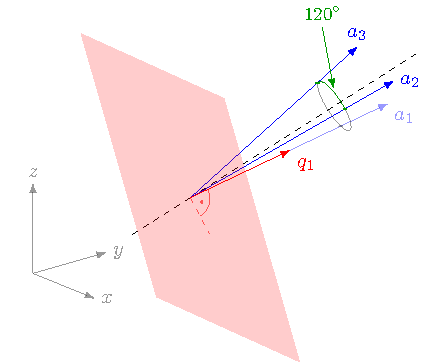
\includegraphics[width=0.45\linewidth]{./papers/qr/pics/gram.pdf}}
	\subfigure[Ganze Zerlegung durchgeführt\label{qr:gram2}]{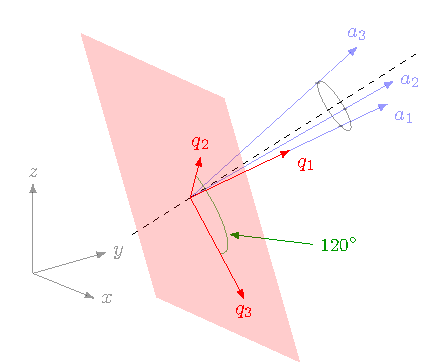
\includegraphics[width=0.45\linewidth]{./papers/qr/pics/gram2.pdf}}
	\caption{Visualisierung von $A$\label{qr:gram}}
\end{figure}
In \ref{qr:gram1} ist ersichtlich, wie die drei Spalten von $A$ jeweils einen Winkel von $120^\circ$ bezüglich der gestrichelten Symmetrielinie einschliessen.
Von den beiden Vektoren $a_2$ und $a_3$ wird jeweils das Skalarprodukt mit $q_1$ abgezogen, danach folgt die normierung, womit man bei \ref{qr:gram2} ist.
Der Winkel $\theta_{23}$ wird in diesem Prozess nie verändert.